Der Luftwiderstand wird vernachlässigt. Die Kapsel hat beim Abwurf die Geschwindigkeit $v_0$ des Flugzeugs in horizontaler Richtung; horizontal fliegt sie gleichförmig weiter, vertikal fällt sie frei.

\begin{abcliste}
\abc Die Falldauer für die Höhe $h$ folgt aus $h = \frac{1}{2}g\,t^2$:
\begin{align}
 t &= \tfF \\
   &= \sqrt{\frac{2\cdot\hf}{\gE}} \\
   &= \tf \approx \result{\tfP{0}{3}}
\end{align}

\abc In dieser Zeit fliegt die Kapsel horizontal die Strecke
\begin{align}
 x &= v_0\,t = \xfF \\
   &= \vfl\cdot\sqrt{\frac{2\cdot\hf}{\gE}} \\
   &= \xf \approx \result{\xfP{3}{2}}
\end{align}
Der Pilot muss die Kapsel also so weit \emph{vor} dem Schiffbrüchigen fallen lassen. Das Flugzeug befindet sich beim Aufprall genau über der Kapsel.

\abc Beim Aufprall ist die vertikale Teilgeschwindigkeit
\begin{align}
 v_y &= \vyfF = \gE\cdot\tf = \vyf
\end{align}
Der Betrag der Aufprallgeschwindigkeit ist
\begin{align}
 v &= \veF \\
   &= \sqrt{\left(\vfl\right)^2+\left(\vyf\right)^2} \\
   &= \ve = \vekP{0}{3} \approx \result{\veP{0}{2}}
\end{align}
\begin{center}
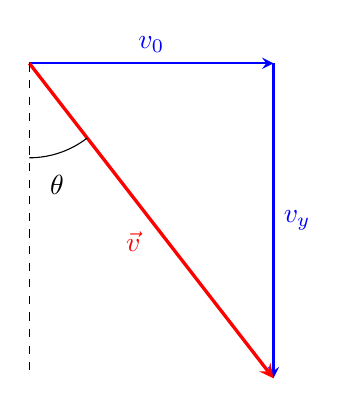
\begin{tikzpicture}[>=stealth]
 \draw[->, thick, blue] (0,0) -- (3.1,0) node[midway, above] {$v_0$};
 \draw[->, thick, blue] (3.1,0) -- (3.1,-4.0) node[midway, right] {$v_y$};
 \draw[->, very thick, red] (0,0) -- (3.1,-4.0) node[midway, below left] {$\vec v$};
 \draw[dashed] (0,0) -- (0,-4.0);
 \draw (0,-1.2) arc[start angle=270, end angle=307.8, radius=1.2];
 \node at (0.35,-1.55) {$\theta$};
\end{tikzpicture}
\end{center}
Für den Winkel $\theta$ gegenüber der Senkrechten (wie in der Abbildung) gilt $\tan\theta = v_0/v_y$:
\begin{align}
 \theta &= \thvF \\
   &= \arctan\frac{\vfl}{\vyf} \\
   &= \thv \approx \result{\thvP{0}{2}}
\end{align}
Gegenüber der Wasseroberfläche trifft die Kapsel also unter $\thhP{0}{2}$ auf.
\end{abcliste}
